\section{The LHC parameters}
\label{s:lhc_param}
The proton beams have a number of associated parameters such as the energy of each beam, 
collision frequency, number of particles in each beam, luminosity etc. An accurate 
and updated knowledge of these parameters is very important during the data taking.
Because they are used in the reconstruction of various physics objects, as well as 
to apply correction on simulated Monte Carlo samples for a better comparison of the 
observed data with simulated results. The information about these parameters is referred to as
\dq{non-event} data since they only contain information about the hardware 
configuration. These parameters are regularly updated on the online master database
system (OMDS). They are later retrieved from the OMDS for offline usage
using dedicated online-to-offline tools. There are thousands of such parameters. 
A few important ones are described below:
\begin{itemize}[leftmargin=*]		
\item $\textbf{The number of particles in each beam}$: One of the basic parameters about the
    	beam is the number of particles in each beam. A proton beam consists of proton
    	bunches. There are nearly 2556 proton bunches in each beam. A typical
	configuration of the bunch is shown in Figure~\ref{subfig:lhc_bunchConf}. There are
    	$1.15\times 10^{11}$ protons in one bunch. Each bunch is separated by 7.5\unit{m} from 
	each other across the LHC ring. The collision frequency of the 
    	bunches is 25\unit{ns}, that is after each 25\unit{ns} counter rotating proton bunches
    	are made to collide at the IP. There is another parameter called
    	\dq{bunches filled for each beam}. It tells out of $2556$ bunches which are filled
    	and which are empty during the data taking. Assuming that all the bunches of
    	a beam are filled, the number of protons in each beam will be 
    	$2556 \times 1.15\times 10^{11} \approx 10^{14}$.
\item $\textbf{Crossing angle ($\alpha$)}$: The $\alpha$ is the angle at which the
	two beams cross at the IP as shown in Figure~\ref{subfig:lhc_xangle}
    	. Its typical value lies in the \unit{$\mu$rad} range. Even though $\alpha$ is 
	very small, a slight change in it affects the number of interactions happening at the
    	collision point. A relatively smaller $\alpha$ implies that the two colliding
    	beams are closer to each other away from the IP. This results in a long-range collision 
	away from the IP. However, a larger value of $\alpha$ reduces the number of collisions as 
	the overlapping area between the beams is smaller.
    	\begin{figure}
    	\centering
      	\subfigure[A typical configuration of proton bunches at the LHC. 
    	\label{subfig:lhc_bunchConf}]
    	{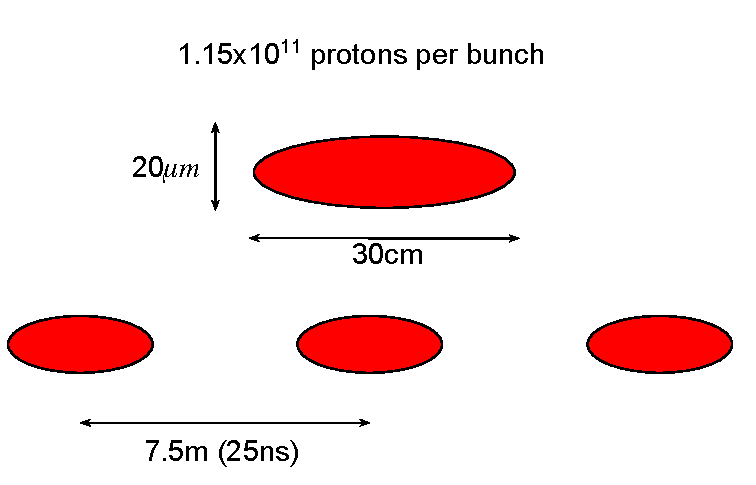
\includegraphics[width=0.49\linewidth]{Experiment/LHC/Image/lhc_bunchConf.pdf}}
    	\hfil
      	\subfigure[The crossing of the beams at the interaction point. 
    	\label{subfig:lhc_xangle}]
    	{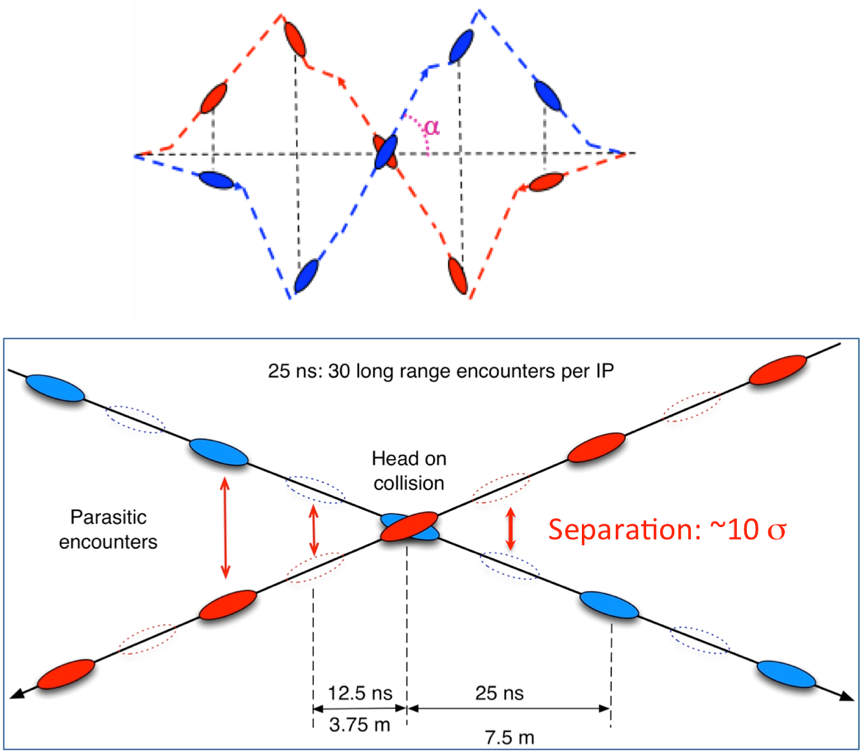
\includegraphics[width=0.49\linewidth]{Experiment/LHC/Image/lhc_xangle.png}}
      	\caption{The bunch configuration and crossing angle. The bunches are separated 
		by 7.5\unit{m}. The crossing angle shown is exaggerated for illustration.
		Figure~\ref{subfig:lhc_bunchConf} is adopted from \cite{CMSDAS} and 
		Figure~\ref{subfig:lhc_xangle} is taken from \cite{Mike}.}
    	\label{subfig:lhc_bunch_xangle}
      	\end{figure}
\item $\textbf{The $\beta^*$}$: The beam sizes do not remain constant throughout the 
	ring. Near the IP, the beams are bent using dipole magnets as shown in 
	Figure~\ref{fig:lhc_beamBend}. Therefore, the beams are a bit squeezed near the IP,  
	the extent of which is quantified with a parameter, called $\beta$. 
	The $\beta^*$ is $\beta$ value at IP. It is the distance from the IP up to a point 
	where the beam size is doubled. 
	The value of $\beta^*$ lies in the \unit{mm} range. Smaller value of $\beta^*$ 
	implies the beam is squeezed near the IP and vice-versa. The formula of $\beta^*$ 
	is given by~\cite{Baird:1017689}
     	\begin{equation}
     		\beta^* = \frac{\pi \sigma^2_{b}}{\epsilon}
     	\end{equation}
     	where $\sigma^2_{b}$ is the cross-sectional size of the bunch and 
	$\epsilon$ is the emittance, the smallest opening a beam
	can be squeezed through ~\cite{Baird:1017689}.
\item $\textbf{Center-of-mass energy ($\sqrt{s}$)}$: The counter rotating protons 
	collide head-on along the z-axis. In the center-of-mass frame, 
	$p_{1z} + p_{2z} = 0$. In addition, the momentum in the transverse plane must be conserved.
	If there is an imbalance in \pt, it would imply the production of some (unknown) particles 
	which has passed the detector without being detected; neutrino is an example. For the two 
	colliding protons with energy $E_1$ and $E_2$, the center-of-mass energy is given by 
	\begin{equation}
		\sqrt{s} = E_1 + E_2
	\end{equation}
     	For the 2016-18 data taking, the energy of each beam was 6.5 \TeV, leading to 
	$\sqrt{s}$ = 13 \TeV. The production of new particles in the physics
	process largely depends on $\sqrt{s}$. Higher the value of $\sqrt{s}$, more is
	the number of produced events for a given process. Many beyond the standard model 
	theories predict the existence of a new particle at higher $\sqrt{s}$. Therefore, 
	the $\sqrt{s}$ is an important parameter of the LHC.
\item $\textbf{Luminosity}$: Like the center-of-mass energy, luminosity is another important 
	parameter which is a measure of how many collisions occur.
	Higher luminosity means a higher chance of producing rare physics process in the
	collisions. With higher luminosity, the standard model predictions can be tested
	with more accuracy thanks to more statistics, hence less uncertainty. It is defined as:  
	\begin{equation}
		L = \frac{1}{\sigma_p}\frac{dR}{dt}
	\end {equation}
	where $\frac{dR}{dt}$ is the number of events per second and $\sigma_p$ is the cross section.
	In the \rm{CGS} unit, the dimension of $L$ is $\unit{cm}^{-2} \unit{s}^{-1}$. However,
	\fbinv (inverse femtobarn) is often used in the collider experiments.
	The luminosity is recorded by experiments over a certain period of time. The
	integrated luminosity is the integration of instantaneous luminosity over a period of time
	\begin{equation}
		L_{\rm{int}} =  \int L dt
	\end{equation}
	At the LHC, the luminosity is calculated in terms of beam parameters such as number of
	particles ($N$), collision frequency ($f$), the number of bunches in the beam ($N_b$), 
	etc \cite{Herr:941318}. 
	\begin{figure}
	  \begin{center}
	  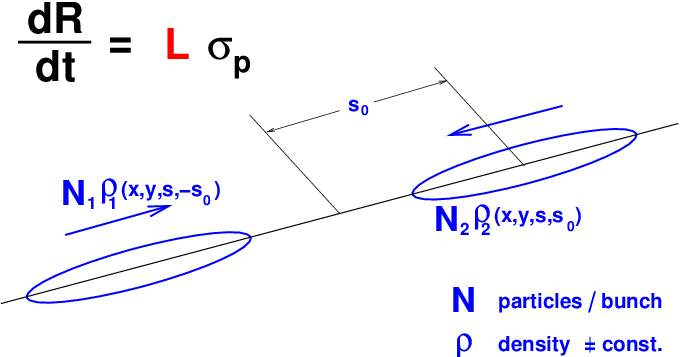
\includegraphics[width=0.50\linewidth]{Experiment/LHC/Image/lhc_lumi.png}
	  \caption{Two oppositely moving bunches with the total number of particles $N_1$ and
		  $N_2$, and beam density distribution functions $\rho_1(x, y, s, -s_0)$ and 
		  $\rho_2(x, y, s, s_0)$
		  \cite{Herr:941318}.}
	  \label{fig:lhc_lumi_rho}
	\end{center}
	\end{figure}
	For two counter rotating bunches with total number of particles 
	$N_1$ and $N_2$, and beam density distribution functions $\rho_1(x, y, s, -s_0)$ and 
	$\rho_2(x, y, s, s_0)$ as shown in Figure~\ref{fig:lhc_lumi_rho}, the luminosity is given 
	by~\cite{Herr:941318} 
	\begin{equation}
		L =  2N_1N_2fN_b\int\int\int\int \rho_1(x, y, s, -s_0) 
		\rho_2(x, y, s, s_0) dxdydsds_0.
	\label{eq:lhc_lumi1}
	\end{equation}
	where $s$ corresponds to the $z$-coordinate which is along the beam direction and $s_0$ is
	the $4^{\rm{th}}$ component of space-time coordinate, that is, $s_0 = ct$. As shown in 
	Figure~\ref{fig:lhc_lumi_rho}, the two bunches meet at $s_0 = 0$. Assuming that the two
	bunches collide head-on and the beam density is uncorrelated along all directions, 
	Equation (\ref{eq:lhc_lumi1}) can be written as
	\begin{equation}
		L =  2N_1N_2fN_b\int\int\int\int \rho_{1x}(x)\rho_{1y}(y)
		\rho_{1s}(s-s_0)\rho_{2x}(x)\rho_{2y}(y)\rho_{2s}(s+s_0) dxdydsds_0.
	\label{eq:lhc_lumi2}
	\end{equation}
 	The beam density distribution at the LHC follows a Gaussian distribution, that is, the 
	proton density is more in the middle of the beam and lesser as one goes away from the
	middle point. Therefore, for the two beams, the beam density functions in 
	Equation (\ref{eq:lhc_lumi2}) can be written as
	\begin{equation}
		\rho_{ix}(x) = \frac{1}{\sigma_{ix}\sqrt{2\pi}}
		\exp\left(-\frac{(x)^2}{2\sigma_{ix}^2}\right), i = 1, 2
	\end{equation}
	\begin{equation}
		\rho_{iy}(x) = \frac{1}{\sigma_{iy}\sqrt{2\pi}}
		\exp\left(-\frac{(y)^2}{2\sigma_{iy}^2}\right), i =1, 2
	\end{equation}
	\begin{equation}
		\rho_s(s\pm s_0) = \frac{1}{\sigma_s\sqrt{2\pi}}
		\exp\left(-\frac{(s\pm s_0)^2}{2\sigma_s^2}\right)
	\end{equation}
	where $\sigma_{ix}$ and $\sigma_{iy}$ are the standard deviation of Gaussian distribution 
	of the two beams along the $x$ and $y$-direction. Using these, Equation (\ref{eq:lhc_lumi2}) 
	becomes \cite{Herr:941318}
	\begin{equation}
		L = \frac{N_1N_2fN_b}{2\pi\sqrt{\sigma_{1x}^2 + \sigma_{2x}^2}
		\sqrt{\sigma_{1y}^2 + \sigma_{2y}^2}}
	\label{eq:lhc_lumi}
	\end{equation}
        Equation (\ref{eq:lhc_lumi}) holds in the ideal situation where the beam profile 
	is uncorrelated in all directions and the machine operates in an ideal condition. However 
	in real life, there are various additional machine effects that need to be 
	incorporated such as finite crossing angle, collision offset, hourglass effect, non-Gaussian 
	beam profiles, nonzero dispersion at the collision point, and so on ~\cite{Herr:941318}. 
	The luminosity given by Equation (\ref{eq:lhc_lumi}) is what delivered by the LHC. Each 
	detector records the luminosity individually during the collision. The recorded luminosity 
	is always smaller than the delivered one due to the detector effects. Five sub-detectors of 
	the CMS experiment are used to monitor and measure the luminosity. These are the silicon 
	pixel detector, the Hadron Forward Calorimeter (HF), the Drift Tubes in the barrel (DT), 
	Pixel Luminosity Telescope (PLT), and  the Fast Beam Conditions Monitor 
	(BCM1f)~\cite{CMS-PAS-LUM-15-001}.

	The luminosity delivered by the LHC and recorded by CMS for 2016 data taking is shown 
	in Figure~\ref{fig:lhc_lumi_2016} over a period of time. The integrated 
	recorded luminosity is 37.8\fbinv for the 2016 data taking. However, a luminosity
	mask is applied to reject some amount where some parts of the CMS detector 
	were not operating in the normal mode. Accordingly, the recorded
	luminosity reduced to 35.9\fbinv. The analysis of 2016 data is what presented in this thesis.
	Delivered luminosity for different center-of-mass energies and during different years
	are shown in Figure~\ref{fig:lhc_lumi_allYear}. The total delivered luminosity at
	13 \TeV during 2015-18 is about 160\fbinv.
	\begin{figure}
       	\centering
      	\subfigure[Delivered luminosity by the LHC and recorded by CMS in 2016 data taking. 
      	\label{fig:lhc_lumi_2016}]
      	      {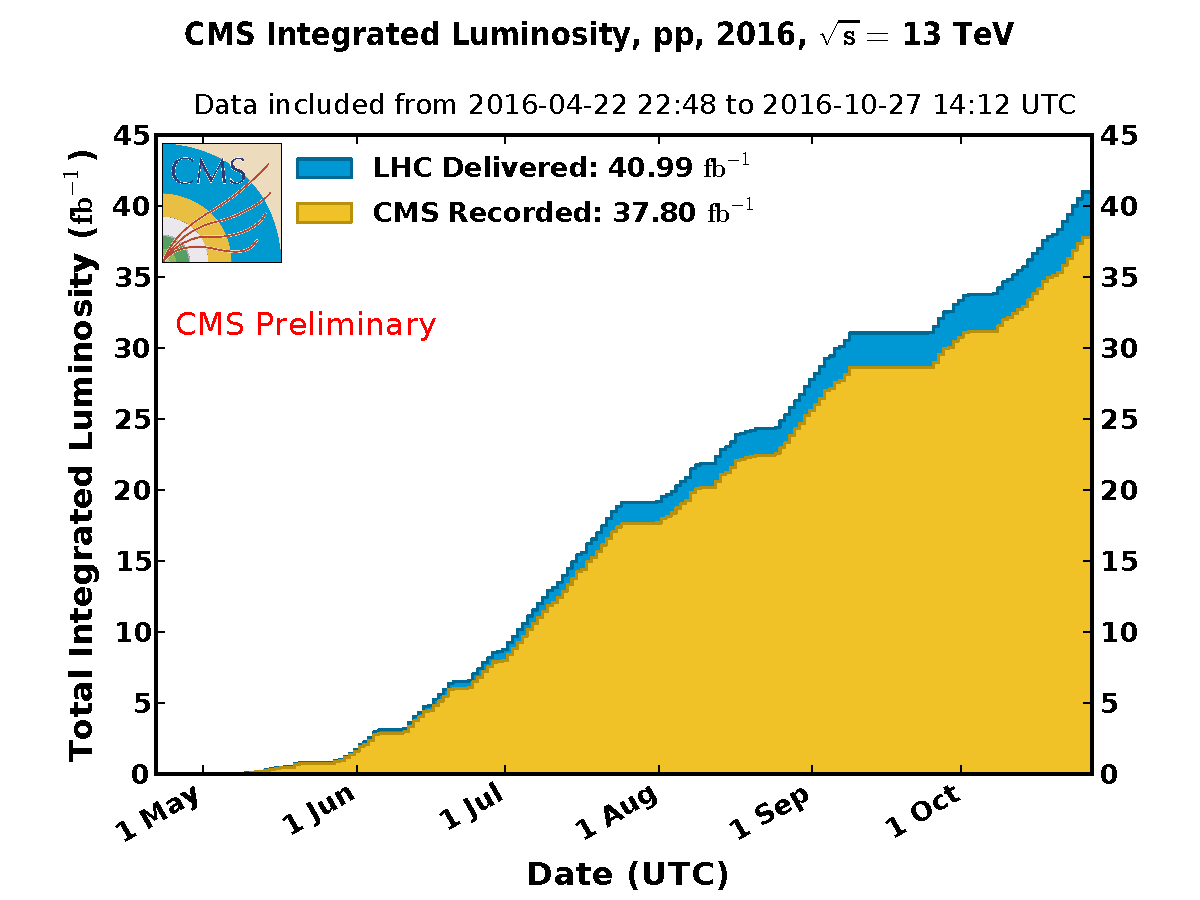
\includegraphics[width=0.49\linewidth]{Experiment/LHC/Image/lumi_2016.pdf}}
      	\hfil
      	\subfigure[Delivered luminosity by the LHC for different years at the different 
	center-of-mass energies, starting from 2010 to 2018.
      	\label{fig:lhc_lumi_allYear}]
	{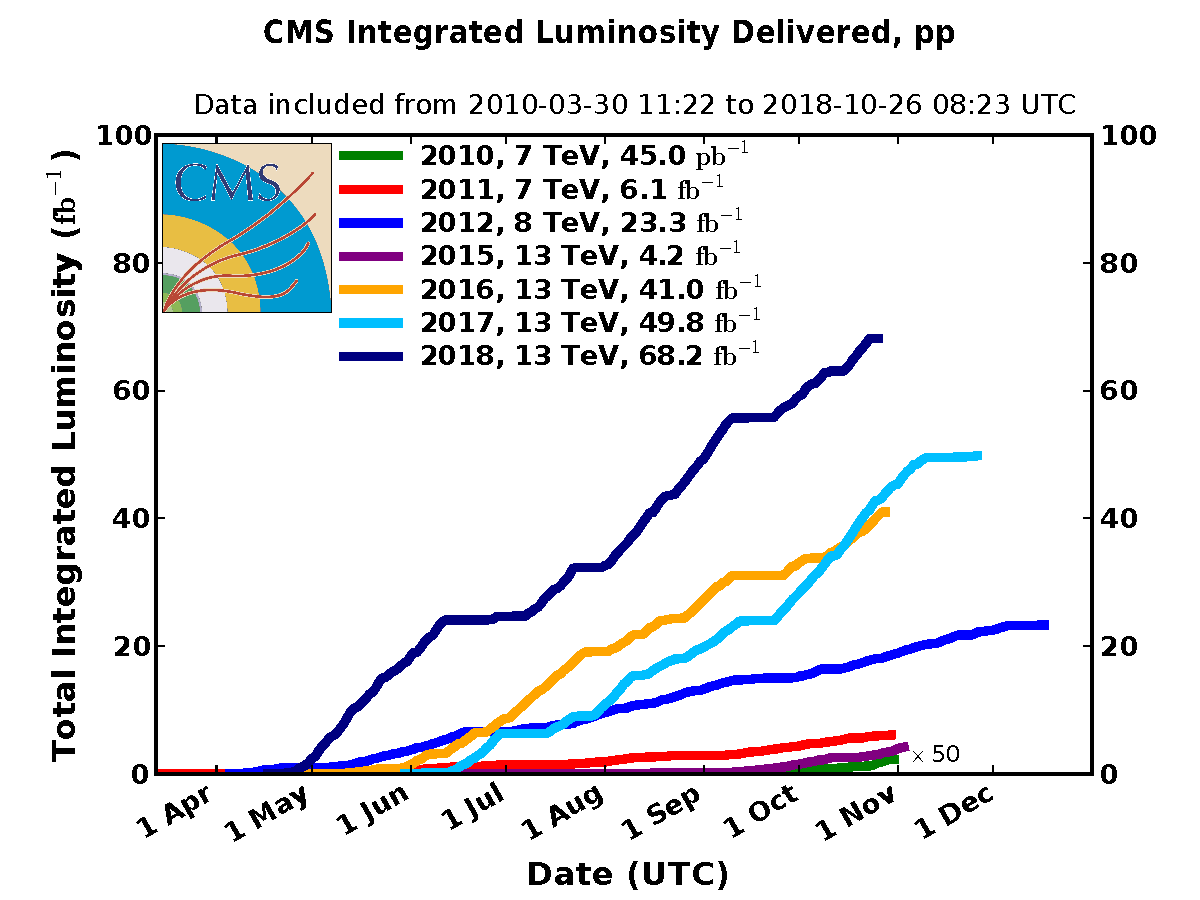
\includegraphics[width=0.49\linewidth]{Experiment/LHC/Image/lumi_allYear.pdf}}
	\caption{Luminosity measurement from different years of the data taking \cite{CMSLumi}. 
		In this thesis, the analysis presented uses the one for the 2016 data taking
		(golden yellow line in the right plot). The total delivered luminosity at 13 \TeV 
		from all years is about 160\fbinv.}
      	\label{fig:lhc_lumi}
     	\end{figure}
\end{itemize}
At the LHC, there are various beam modes indicating the beam status such as 
\dq{Squeeze} (the beams are squeezed by betatron towards the target collision, for most of
the 2016 data taking the $\beta^*$ = 30\unit{cm}), \dq{Adjust} (the separation between the beams
is made to collapse, bringing them for collision), \dq{Stable beams} (it signals that
the physics data taking can be started), and \dq{Dump} (the beams are dumped after the data
taking ends). The stable beam mode lasts for a few hours during which the collisions are recorded.

A \dq{Fill} is created as soon as the stable beams are achieved and all the detector information
is updated in the online database. A Fill lasts for few hours and is divided in 
\dq{Runs} for better management. Further, a Run is divided in \dq{lumi sections}. The duration
of each lumi section (LS) is 23\unit{s}. Therefore, the data taking by a detector has a granularity
of 23\unit{s}. That is, the detector information is updated/stored after each 23\unit{s}. An LS 
is marked as good or bad depending on whether all the parts of the detector were
on or some of them were off. The integrated luminosity is obtained by summing over all LS.

All the LHC parameters are measured regularly during the data taking. Most of them
do not change on a regular day-to-day basis. However, few do change on every day during the data
taking such as the ones shown in Figure~\ref{fig:lhc_param_day}. Other parameters change over
a period of time, for example on a month-to-month basis, and some even on a yearly basis
such as the ones shown in Figure~\ref{fig:lhc_param_month}.

\begin{figure}
  \begin{center}
  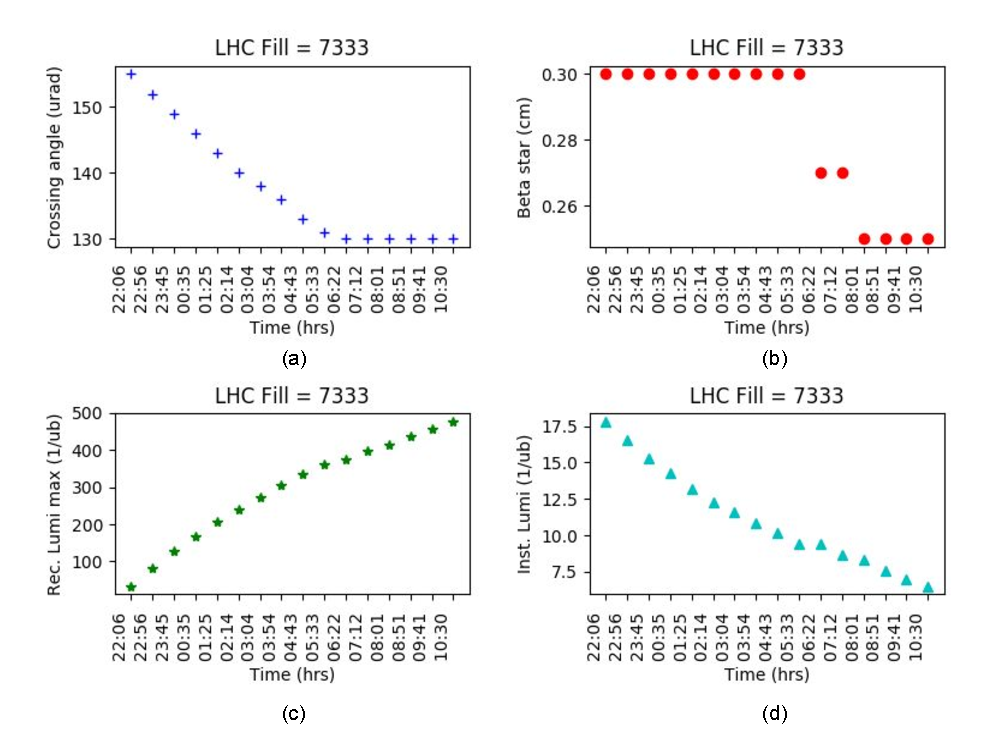
\includegraphics[width=0.70\linewidth]{Experiment/LHC/Image/lhc_param_day.pdf}
  \caption{Variation of few LHC parameters during the data taking on 22-23rd October
	  2018 (Fill = 7333). All these parameters change over a different point of time.
	  Other parameters such as the center-of-mass energy, number of particles in 
	  each beam, etc do not change on a given day.
	  }
  \label{fig:lhc_param_day}
  \end{center}
\end{figure}
\begin{figure}
  \begin{center}
  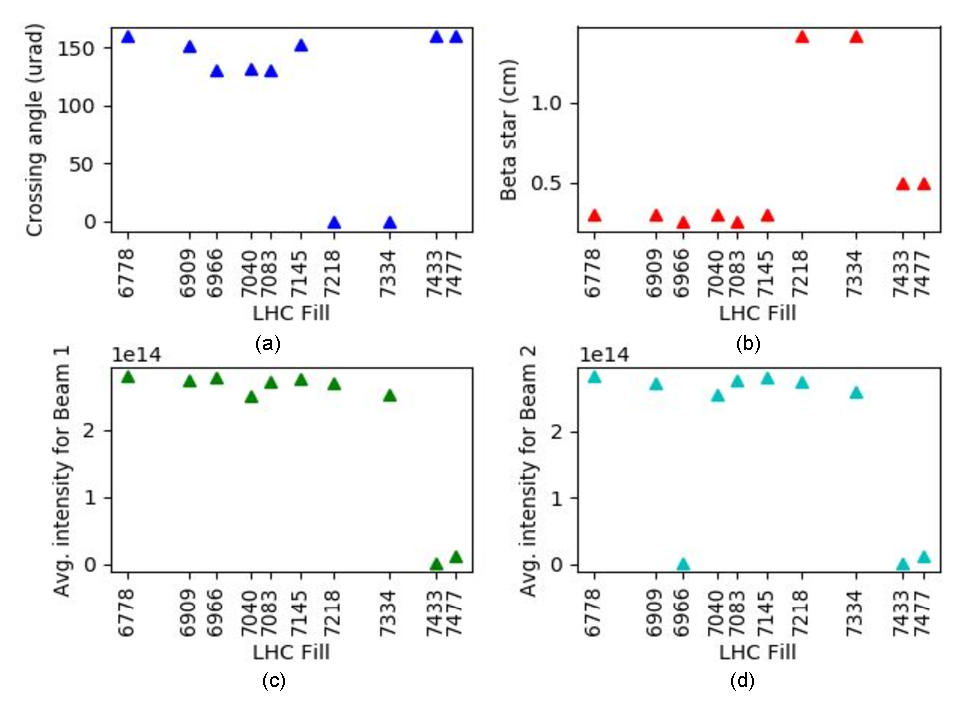
\includegraphics[width=0.70\linewidth]{Experiment/LHC/Image/lhc_param_month.pdf}
  \caption{Variation of few LHC parameters during the data taking from random days in
	  the period of June-November 2018. Only a few days (Fills) have been chosen for
	  illustration. The last two Fills (7433 and 7477) correspond to Pb-Pb, 
	  rest are from proton-proton collisions. The average intensity of the beam is the 
	  number of particles in each beam. As can be seen, all these parameters change over 
	  a different period of time.
	  }
  \label{fig:lhc_param_month}
  \end{center}
\end{figure}
